\documentclass[a4paper,11pt]{article}
\usepackage[utf8]{inputenc}
\usepackage{graphics}
\usepackage{amssymb}
\usepackage{geometry}
\usepackage{complexity}
\usepackage{amsmath}
\geometry{a4paper, margin=1in}
\usepackage[export]{adjustbox}
\usepackage{hyperref}
\hypersetup{
    colorlinks=true,
    linkcolor=blue,
    filecolor=magenta,      
    urlcolor=blue,
}
\urlstyle{same}
\graphicspath{ {./images/} }
\everymath{\displaystyle}
\setlength{\parskip}{1em}
\setlength{\parindent}{0em}
\usepackage{setspace}
\title{CS 451: Computational Intelligence \\ \Large Final Project}
\author{Proposal}
\date{\today}

\begin{document}
\maketitle
\begin{center}
    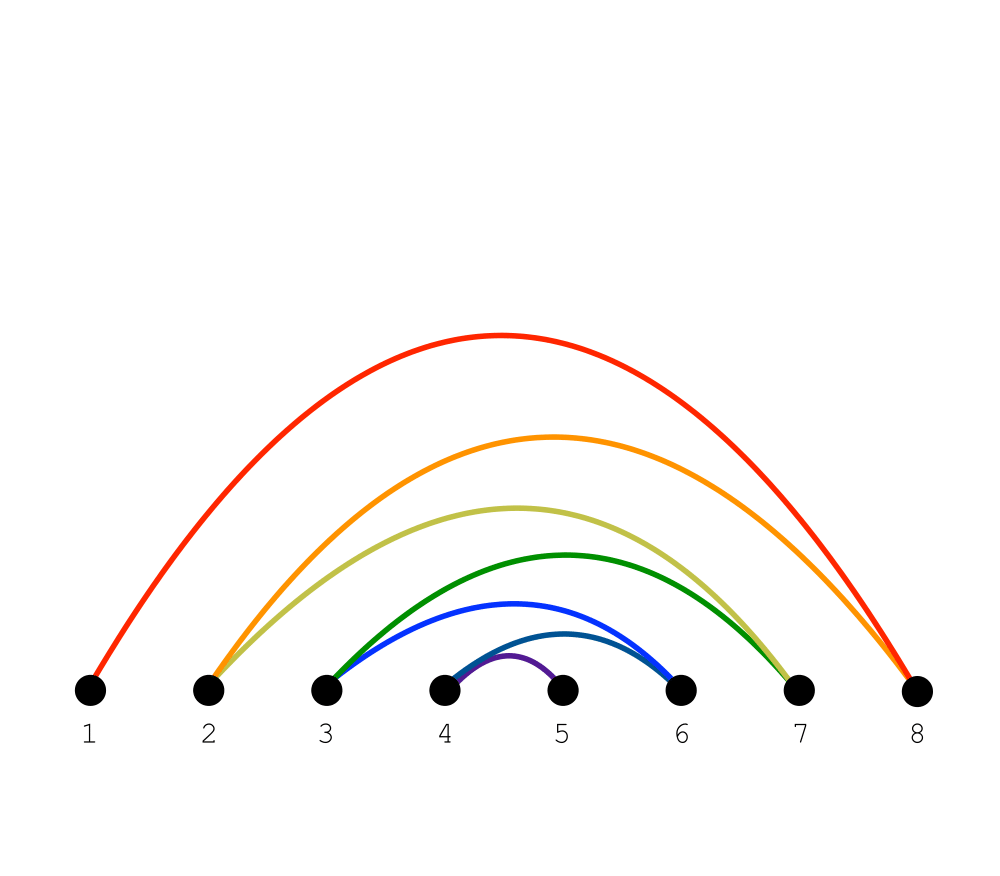
\includegraphics[scale=0.4]{cover.png}    
\end{center}


\newpage
\begin{spacing}{0.01}
    \tableofcontents
\end{spacing}


\newpage
\section{Introduction \& Logistics}
\textbf{Topic:} Graph Bandwidth Problem 

\textbf{Section:} L1 - Dr. Saleha Raza 

\textbf{Group Members:} 
\vspace{0.4 em} \\
*All names appear in alphabetical order; any other apparent pattern is purely coincidental.
\begin{enumerate}
    \item Maaz Saeed - ms05050
    \item Maham Shoaib Patel - mp04911
    \item Muhammad Usaid Rehman - mr04302
\end{enumerate}

\textbf{GitHub Repository:} \url{https://github.com/m-usaid/CS451-FinalProject}

\section{Graph Bandwidth Problem}

The bandwidth problem for a graph $G = (V,E)$ to label its $|V|$ vertices $v_i \in V(G)$ with distinct integers such that the quantity max$\{|f(v_i) - f(v_j)|: v_iv_j \in E(G)\}$ is minimized. The problem is concerned with the linear ordering of vertices. 

The weighted variant of the problem has an extra component and our objective function becomes:
\[\text{max}\{w_{ij}|f(v_i)-f(v_j)| : v_iv_j \in E(G)\}.\]
The problem aims to minimize the maximum `stretch' that any edge would have in a linear ordering of the graph. If we were to put the vertices of the graph on unique integer points of
of the $x$-axis, then the length of the longest edge should be minimized. 

This problem is closely related to the general bandwidth problem for matrices. In fact, the graph bandwidth of the symmetric matrix is the bandwidth of the symmetric matrix which is the adjacency matrix of the graph.


\subsection{Problem Definition}
Let's define the problem in more formal terms with some added notation. 
The mapping $f$ is defined as $f: V(G) \to \{1, 2, \dots, n\}$, where $n = |V|$ -- also called a \emph{perfect numbering}. \cite{Lee2016} Therefore, 
we can think of these mappings as essentially orderings of the vertices. The bandwidth of an ordering is defined as:
\[B_f(G) = \text{max}_{uv \in E(G)}\{|f(u) - f(v)|\}.\]
The bandwidth of the graph $G$ is given by the bandwidth of the best possible ordering:
\[B(G) = \text{min}\{B_f(G): f \text{ is a numbering of }G\}.\]
We will be restricting ourselves to working with perfect numberings.

\newpage
\subsection{Runtime Complexity \& Approximation Algorithms}
Previous research has proven the intractability of the graph bandwidth problem. Papadimitrou showed that the problem is $\NP$-complete in \cite{papadimitriou_1976}. There are some special cases of the problem where an exact solution can be obtained in polynomial time; however, there has been no successful attempt to find a solution for a general case. 

It is also pertinent to note that the bandwidth is also $\NP$-hard to approximate with any 
$O(1)$-approximation algorithms. For general cases, not much work has been done to find 
approximation algorithms for the problem -- owing to the hardness of approximation. 

On that note, we turn our attention to heuristic algorithms. There are several heuristic 
algorithms for the bandwidth problems such as the Cuthill-McKee algorithm, and the 
Gibbs-Poole-Stockmeyer algorithm. Heuristic approaches are of interest to us since they will give us an idea as to how we can design appropriate meta-heuristic techniques to solve 
the bandwidth problem. 

\section{Motivation}
The graph bandwidth problem is relatively new and inadequately researched as compared to other NP hard graph problems. The solution to the graph bandwidth problem using evolutionary algorithm and analysis is largely unexplored. Since the problem is both $\NP$-hard to solve and $\NP$-hard to approximate, we believe that evolutionary
approaches are the next best step and will lead to interesting results. 
The prospect of solving a graph problem using EA incurs deep curiosity and it is why we have chosen to pursue this topic.

Since the graph bandwidth is a special case of the quadratic bottleneck assignment problem, it will be interesting to also utilize ant-colony optimization (ACO) to obtain results for the problem. It will also allow us to compare results with evolutionary algorithm and provide a comprehensive comparative analysis.

\section{Related Work}
Most of our theoretical study of the problem and the nature of its intractability has come from \cite{ccdg1982} and \cite{garey_johnson_2003}. 
Knowledge about the hardness of approximation came from \cite{743431}.  \cite{beineke_wilson_1983} gave a holistic overview of the problem. 

Other than this, we will be relying on the course textbooks -- \cite{nunes_2023} \& \cite{engelbrecht_computational_2007} to learn more about ACO and EA in order to implement them. We will be relying on \href{http://people.brunel.ac.uk/~mastjjb/jeb/orlib/}{this data-set} to get
information to create instances of large graphs to test our algorithms on. 

There is not a lot of research work that is directly tied to the work that 
we want to do since the topic is fairly niche. Therefore, we think that our work will be more interesting owing to the lack of preexisting data. 
\section{Outcomes}
We plan to solve the algorithm by deriving a meta-heuristic solution to the problem set using python libraries;NetworkX, and NumPy. Our objectives revolve around trying to  determine whether the problem can be solved using evolutionary algorithms and/or ACO algorithms. Additionally we plan to provide a detailed comparative analysis on the results derived through the two methods.

\bibliographystyle{ieeetr}
\bibliography{refs.bib}

\end{document}